%%%%%%%%%%%%%%%%
% Class
%%%%%%%%%%%%%%%%

	\documentclass[openany,letterpaper,final]{book}
	
%%%%%%%%%%%%%%%%
% Packages
%%%%%%%%%%%%%%%%

	\usepackage{fancyhdr}
	\usepackage[margin=1in]{geometry}
	\usepackage{graphicx}
	\usepackage{amsmath}
	\usepackage{pdflscape}
	\usepackage{tikz}
	\usetikzlibrary{shapes}
	\usetikzlibrary{decorations}
	\usetikzlibrary{decorations.pathreplacing}
	\usetikzlibrary{decorations.pathmorphing}
	\usepackage{titlesec}
	\usepackage{hyperref}
	\hypersetup{pdftex,colorlinks=true,allcolors=black}
	\usepackage{hypcap}

%%%%%%%%%%%%%%%%
% Other opts and styling
%%%%%%%%%%%%%%%%

	\graphicspath{{./assets/}}
	
	% Page headers
	\pagestyle{fancy}
	\renewcommand{\headrulewidth}{0pt}
	\fancyhead{}
	\fancyfoot{}
	\rhead{\thepage}

	% Chapter styling
	\titleformat{\chapter}
	{\normalfont\LARGE\bfseries}{\thechapter}{1em}{}
	\titlespacing*{\chapter}{0pt}{3.5ex plus 1ex minus .2ex}{2.3ex plus .2ex}
	
	% ToC depth
	\setcounter{tocdepth}{2}

%%%%%%%%%%%%%%%%
% BEGIN DOCUMENT
%%%%%%%%%%%%%%%%

	\begin{document}

%%%%%%%%%%%%%%%%
% New commands
%%%%%%%%%%%%%%%%
	
	% Thick horizontal rule
	\newcommand{\HRule}{\rule{\linewidth}{0.5mm}}
	
	% Easy scientific notation
	\newcommand{\e}[1]{\ensuremath{\times 10^{#1}}}

%%%%%%%%%%%%%%%%
% TITLE PAGE
%%%%%%%%%%%%%%%%

	%!TEX root=./labNotes.tex

\begin{titlepage}
	{~ \\[5cm] }
	
	\noindent \HRule \\[0.4cm]
	{ \Huge \bfseries McDonald Lab \\[0.4cm] }
	{ \huge \bfseries Lab Protocols and Daily Log \\ }
	\HRule \\[0.4cm]
	
	\noindent { \Large Christopher Wetherill \\[0.15cm] }
	{ \large \emph{Virginia Polytechnic Institute and State University} }\\[11cm]
	
	\noindent Audit log available at https://github.com/faulconbridge/TBMH/tree/master/Rotations
\end{titlepage}

%%%%%%%%%%%%%%%%
% FRONTMATTER
%%%%%%%%%%%%%%%%

	\tableofcontents
	
%%%%%%%%%%%%%%%%
% CONTENTS
%%%%%%%%%%%%%%%%

	%%%%%%%%%%
	% Overview
	%%%%%%%%%%	
	%!TEX root=./virology.tex

\section{Lab Protocols}

\subsection{Location of Common Materials}

\begin{tabular*}{\textwidth}{r | p{2in} p{2in}}
\hline
Item & Location & Storage \\
\hline
(In)complete Medium 199 & Incomplete Medium 199 is located in the cold room in the hallway immediately outside the lab. & Complete and serum-free Medium 199s are stored in the $4^{\circ}$C freezer in R2048.\\
Penicillin/Streptomycin Stock & P/S stock is located in the $-20^{\circ}$C freezer in the hallway immediately outside the lab. & Leftover stock is stored in the $4^{\circ}$C freezer in R2048.\\
L-Glutamine Stock & Stock is located in the $-20^{\circ}$C freezer in the hallway immediately outside the lab. & Leftover stock is stored in the $4^{\circ}$C freezer in R2048.\\
Amphotericin B stock & Stock is located in the $-20^{\circ}$C freezer in the hallway immediately outside the lab. & Leftover stock is stored in the $4^{\circ}$C freezer in R2048.\\
0.05\% Trypsin-EDTA & Stock is located in the $-20^{\circ}$C freezer in the hallway immediately outside the lab. & Leftover stock is stored in the $4^{\circ}$C freezer in R2048.\\
Fetal Bovine Serum & Stock is located in the $-20^{\circ}$C freezer in the hallway immediately outside the lab. & Leftover stock is stored in the $4^{\circ}$C freezer in R2048.\\
(In)complete 2x EMEM & Stock is located in the cold room in the hallway immediately outside the lab. & Complete EMEM stock is stored in the $4^{\circ}$C freezer in R2048.\\
SeaPlaque Agarose & Stock is located in a jar above the benches immediately outside of the biosafety cabinet. & Leftover stock should be replaced where you found it.\\
\hline
\end{tabular*}

\subsection{Recording Work and Labelling Materials}

All solutions should be labeled with your name, the date of preparation, and what the solution contains. All cell flasks should be labeled with your name, the date of preparation, the type of cell contained, and the passage of cell contained.

All work completed in the lab should be recorded in a laboratory notebook. Each page should contain entries from only a single day. The date of entry should be recorded at the top of each page. All writing must be easily readable and written in pen. Any errors should be struck through with a single solid line with the correction appearing next to it. Any space on a page not used at the end of a work day should be clearly crossed out in pen.

\subsection{Preparation of Medium 199 (Serum-Free)}

{\bfseries Items Needed:}\footnote{The paper {\itshape Culturing, Storage, and Quantification of Rotaviruses} advises using different quantities of some materials below. Nonetheless, the following are the recommended quantities for use in lab.} \begin{enumerate}
	\item Incomplete Medium 199 ($500$mL)
	\item Penicillin/streptomycin stock ($5$mL)
	\item Amphotericin B stock ($1$mL; $250\mu$g/mL)
\end{enumerate}

In the biosafety cabinet, supplement $500$mL incomplete Medium 199 with $5$mL P/S stock and $1$mL amphotericin B stock. Store at $4^{\circ}$C for up to 3 months.

\subsection{Preparation of Medium 199 (Complete)}

{\bfseries Items Needed:}\footnote{See Note 1.} \begin{enumerate}
	\item Incomplete Medium 199 ($500$mL)
	\item Penicillin/streptomycin stock ($5$mL)
	\item Amphotericin B stock ($1$mL; $250\mu$g/mL)
	\item Fetal bovine serum ($55$mL)
\end{enumerate}

In the biosafety cabinet, supplement $500$mL incomplete Medium 199 with $5$mL P/S stock, $1$mL amphotericin B stock, and $55$mL fetal bovine serum. Store at $4^{\circ}$C for up to 3 months.

\subsection{Preparation of 1.2\% Agarose}

{\bfseries Items Needed:} \begin{enumerate}
	\item SeaPlaque agarose
	\item Milli-Q filtered water
\end{enumerate}

To a $500$mL flask add $1.2$g agarose for every $100$mL water. Inadvisable to fill flask to more than $400$mL. Cap and shake. Loosen lid. Apply autoclave tape to the lid. Autoclave approx. 20 min.

\subsection{Preparation of 2x EMEM (Serum-Free)}

{\bfseries Items Needed:} \begin{enumerate}
	\item incomplete 2x EMEM ($500$mL)
	\item $200$mM \textsc{l}-glutamine ($10$mL)
	\item P/S stock ($10$mL)
	\item $250\mu$g/ml amphotericin B stock ($1$mL)
\end{enumerate}

In the biosafety cabinet, to incomplete 2x EMEM stock add \textsc{L}-glutamine, P/S stock, and amphotericin B stock. Store at $4^{\circ}$C for up to 3 months.

\subsection{Preparation of PBS (Phosphate Buffered Saline)}

\subsection{Procedure for Splitting MA104 Cells}

{\bfseries Items Needed:} \begin{enumerate}
	\item 1x PBS
	\item 0.05\% Trypsin-EDTA
	\item Complete Medium 199
	\item $150$cm$^2$ flask
\end{enumerate}

In a water bath, warm PBS, Trypsin, and complete Medium 199 to $37^{\circ}$C. Transfer all materials into the biosafety cabinet. Tilt the flask with your cells (having formed a confluent monolayer) such that the culture medium collects on the sloped surface leading to the neck of the flask. Vacuum out all culture medium using a small glass pipet inserted into the rubber vacuum hose. To the cell culture, add $5$mL Trypsin, tilting the flask forward and back to ensure that the cells are fully bathed. Vacuum out the Trypsin.

Add a second $5$mL portion of Trypsin to the cell culture. Incubate at $37^{\circ}$C until all cells have detached from the surface and are free-floating. Lightly tap the flask with your hand if any cells remain attached. Add $15$mL complete Medium 199. (If you used less trypsin in the previous step, adjust the amount of Medium 199 applied such that there is $20$mL solution in the flask.)

To each new flask that you wish to prepare, add complete Medium 199 such that the final flask volume after the cell mixture is added will be equal to $25$mL. To determine the volume of cell mixture to add to each new flask, we use Table 1.1.

\begin{figure}[htp]
{\bfseries Table 1.1}\\[0.1cm]
\begin{tabular*}{\textwidth}{c c}
\hline
Cell dilution ratio & Cell mix volume to add \\
\hline
1:2 & 10mL \\
1:4 & 5mL \\
1:8 & 2.5mL \\
\hline
\end{tabular*}\\[0.1cm]
{\small {\itshape Note.} For example, if we wished to prepare one 1:4 dilution and two 1:8 dilutions, to our first flask we would add 15mL complete Medium 199 and 10mL cell mixture; to each of our second two flasks we would add 20mL complete Medium 199 and 5mL cell mixture.}
\end{figure}

Cap the new flask(s) and tilt forward and back to evenly spread the cells. Loosen the lids and incubate at $37^{\circ}$C.

\subsection{Procedure for Plating MA104 Cells}

\subsection{Procedure for activating RV SA11 and Infecting MA104 Cells}

\subsection{Procedure for Performing RV Plaque Assay}

\subsection{Procedure for Transducing MA104 Cells with siRNA-Expressing Lentiviral Vectors}
	\clearpage
	
	%!TEX root = ./virology.tex

\section{Rotavirus}

\subsection{History}

Human rotavirus (RV) was discovered in 1973 by Bishop et al. utilizing direct visualization by electron microscopy. Approximately concurrently, simian, murine, O, and bovine agents were discovered that later would be additionally classified as rotaviral.

\subsection{Classification}

RVs comprise the genus \textit{Rotavirus} within the family \textit{Reoviridae}. Some features are that:

\begin{enumerate}
	\item the mature viruses are about $100$nm ($1,000$\AA) in diameter with a triple-layered icosahedral protein capsid being comprised of outer and intermediate layers and an inner core;
	\item 60 protein spikes protrude from the outer shell;
	\item calcium is required to maintain the integrity of the outer shell;
	\item particles contain an RNA-dependent RNA polymerase and related enzymes able to produce capped RNA transcripts;
	\item the virus genome contains 11 dsRNA segments;
	\item genetic reassortment can occur between two rotaviruses of the same group; and
	\item the virus particles, uniquely, are formed by migration into the ER where enveloped particles are formed.
\end{enumerate}

RVs are classified into serogroups of multiple serotypes each. An RV group includes viruses that share cross-reacting antigens. There are 7 distinct groups that rotaviruses compose. Group A, B, and C RVs are found in both humans and animals; group D, E, F, and G RVs have only been observed in animals to date.

Group A RVs have been predominantly identified as causing diarrheal disease in infants and mammalian and avian young. Group B RVs are associated with severe diarrheal epidemics. Group C RVs have been occasionally reported in family outbreaks.

\clearpage
\begin{landscape}
{\bfseries \large Table 2.1} \\[0.1cm]
\begin{tabular}{rr|lllp{4.5in}}
\hline
\parbox[t]{0.5in}{Genome\\Segment} & \parbox[t]{0.55in}{Protein Product} & Location & N/virion & \parbox[t]{0.7in}{Ts mutant group} & Function \\
\hline
1 & VP1 & Core & 12 & C & RNA-dependent RNA polymerase, ss-RNA binding, complex with VP3 \\
2 & VP2 & Core & 120 & F & RNA binding, required for replicase activity of VP1 \\
3 & VP3 & Core & 12 & B & Guanylytransferase, methytransferase, ss-RNA binding, complex with VP1 \\
4 & VP4 & Outer capsid & 120 & A & Hemagglutinin, cell attachment, neutralization antigen, protease enhanced infectivity, virulence, putative fusion region \\
5 & NSP1 & Nonstructural & & NA & Basic, zinc finger, RNA binding, virulence in mice; interacts with and degrades IRF-3; nonessential for some strains \\
6 & VP6 & Inner capsid & 780 & G & Hydrophobic, trimer, subgroup antigen, protection; required for transcription \\
7 & NSP3 & Nonstructural & & NA & Acidic dimer, binds $3^{\prime}$ end of viral mRNAs, competes with cellular PABP for interaction with elF-4G1, inhibits host translation \\
8 & NSP2 & Nonstructural & & E & Basic, RNA binding, oligomer, NTPase, helicase, forms viroplasms with NSP5 \\
9 & VP7 & Outer capsid & 780 & NA & RER integral membrance glycoprotein, calcium-dependent trimer, neutralization antigen \\
10 & NSP4 & Nonstructural & & NA & RER transmembrance glycoprotein, intracellular receptor for DLPs, role in morphogenesis, interacts with viroplasms, modulates intracellular calcium and RNA replication, enterotoxin, secreted cleavage product, protection by antibody, virulence \\
11 & NSP5 & Nonstructural & & NA & Basic phosphoprotein, RNA binding, protein kinase, forms viroplasms with NSP2, interacts with VP2 and NSP6 \\
& NSP6  & Nonstructural & & NA & Interacts with NSP5, present in viroplasms and most virus strains \\
\hline
\end{tabular} \\[0.1cm]
{\itshape Note.} Table of rotavirus proteins and their relevant data. Adapted from Fields Biology, 5e.
\end{landscape}
\clearpage

\subsection{Virion Structure}

Three-dimensional reconstructions using cryo-electron microscopy have revealed that RV particles possess icosahedral symmetry with a $T=13l$ icosahedral surface lattice for the two outer layers. There exist also $132$ large channels $\sim 140\AA$ deep that span both shells and link the outer surface with the inner core. The virion is schematically represented in Figure \ref{fig01}).

\begin{figure}[htp]
\begin{center}
% Define decoration
\pgfdeclaredecoration{outerCapsid}{initial}
{
  \state{initial}[width=\pgfdecoratedpathlength/floor(\pgfdecoratedpathlength/7pt)]
  {
    % Draw the two legs
    \pgfpathmoveto{\pgfpoint{-1pt}{0pt}}
    \pgfpathlineto{\pgfpoint{-1pt}{-10pt}}
    \pgfpathmoveto{\pgfpoint{1pt}{0pt}}
    \pgfpathlineto{\pgfpoint{1pt}{-10pt}}
    % Draw the head group
    \pgfpathmoveto{\pgfpoint{1pt}{0pt}}
    \pgfpathcircle{\pgfpoint{0pt}{2pt}}{2.5pt}
  }
  \state{final}
  {
    \pgfpathmoveto{\pgfpointdecoratedpathlast}
  }
}

\pgfdeclaredecoration{intermediate}{initial}
{
  \state{initial}[width=\pgfdecoratedpathlength/floor(\pgfdecoratedpathlength/7pt)]
  {
	\draw [fill = red!50] (2pt,3pt) -- (-2pt,3pt) -- (-1pt, 0pt) -- (-2pt, -3pt) -- (2pt, -3pt) -- (1pt, 0pt) -- cycle;
  }
  \state{final}
  {
    \pgfpathmoveto{\pgfpointdecoratedpathlast}
  }
}

\pgfdeclaredecoration{inner}{initial}
{
  \state{initial}[width=\pgfdecoratedpathlength/floor(\pgfdecoratedpathlength/8pt)]
  {
\draw [fill = blue!50] (2.5pt,0pt) -- (0pt,2.5pt) -- (-2.5pt,0pt) -- (0pt,-2.5pt) -- cycle;
  }
  \state{final}
  {
    \pgfpathmoveto{\pgfpointdecoratedpathlast}
  }
\pgfusepath{fill,stroke}
}

\begin{tikzpicture}
% Rotavirus
\draw[decorate, decoration={inner}] (5, 0.5) circle (2.5cm);
\draw[decorate, decoration={intermediate}] (5, 0.5) circle (2.8cm);
\draw[decorate, thick] (5, 0.5) circle (2.95cm);
\draw[decorate, fill=green, decoration={outerCapsid, mirror}] (5, 0.5) circle (3.3cm);
\draw[decorate, decoration={coil, aspect=0, segment length=0.5cm, amplitude=.15cm}] (3.1,0) -- (5.5,0);
\draw[decorate, decoration={coil, aspect=0, segment length=0.5cm, amplitude=-.15cm}] (3,0) -- (5.5,0);
\draw[decorate, decoration={coil, aspect=0, segment length=0.5cm, amplitude=.15cm}] (4.1,1.5) -- (6.5,1.5);
\draw[decorate, decoration={coil, aspect=0, segment length=0.5cm, amplitude=-.15cm}] (4,1.5) -- (6.5,1.5);
\draw (6.3,1.4) -- (10,1.4);
\node at (10.75,1.4) {dsRNA};
\draw (8.5,0) -- (10,0);
\node at (12.1,0) {Embedded protein spike};
\draw (7.8,-0.6) -- (10,-0.6);
\node at (11.15,-0.6) {Outer capsid};
\draw (7.3,-1.15) -- (10,-1.15);
\node at (11.78,-1.15) {Intermediate capsid};
\draw (6.1,-1.75) -- (10,-1.75);
\node at (11.15,-1.75) {Inner capsid};
\end{tikzpicture}\\[1cm]
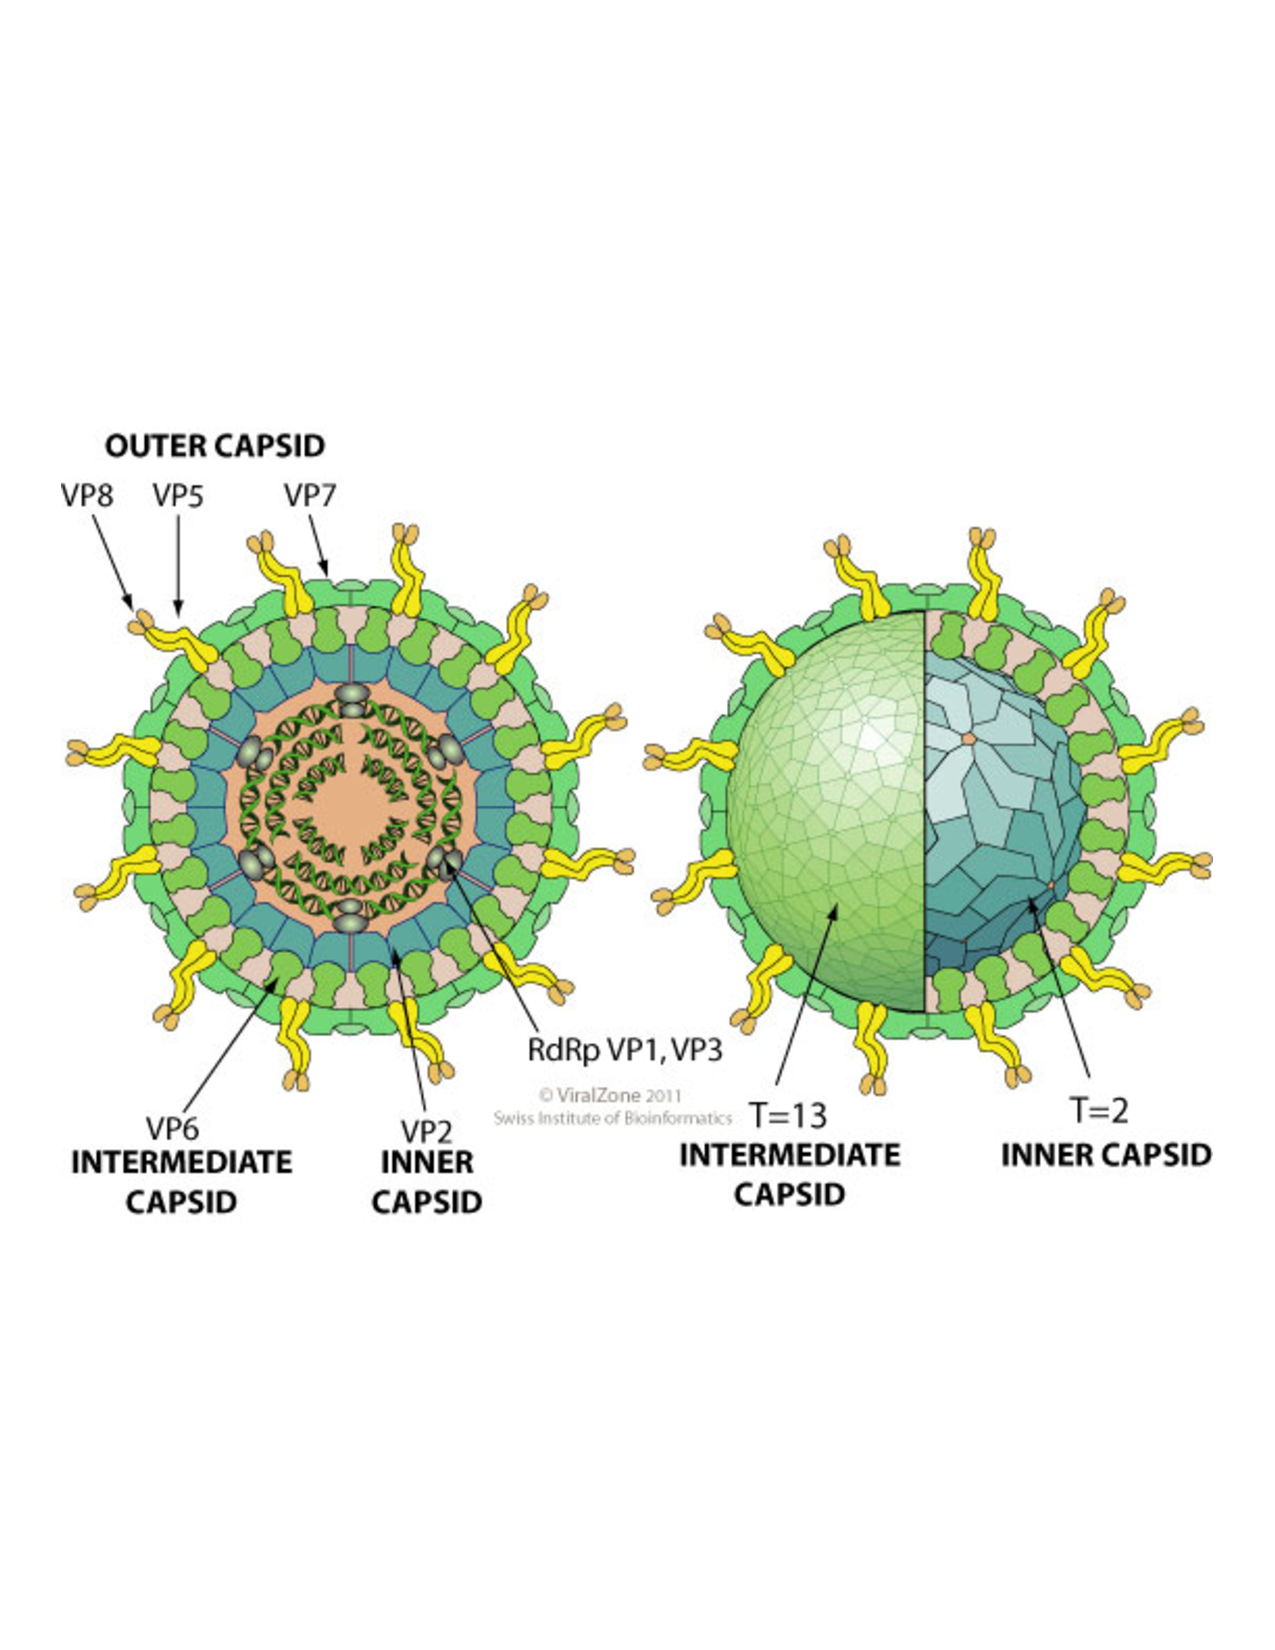
\includegraphics[width = 6in]{virion}
\end{center}
\caption{Schematic illustration of a rotavirus particle, laterally bisected (top) accompanied by an alternate representation showing the specific structural proteins (bottom left). The structures of the virion's three capsids is also represented (bottom right).}
\label{fig01}
\end{figure}

Three types of channels have been identified based on position and size. Specifically, there are $12$ type I channels running down the icosahedral fivefold axes; 60 type II channels around the fivefold axes; and 60 type III channels around the threefold icosahedral axes.

Further, 60 spikes extend from the surface of he outer shell. These protein spikes lit on the edges of the type II channels and are composed of VP4. The spikes have a distinct structure with two distal globular head domains, a central body, and an internal globular domain tucked inside the VP7 layer in the type II channels.  

\subsection{Genome Structure}

The viral genome of 11 dsRNA segments is contained within the core capsid. The virus particles have been shown to contain their own RNA-dependent RNA polymerase to transcribe the individual RNA segments into active mRNA. (I.e., deproteinized RV dsRNA are non-infectious.)

Each positive-sense RNA segment starts with a $5^{\prime}$-guanidine followed by a set of conserved sequences that are part of the $5^{\prime}$-noncoding sequences. An open reading frame (ORF) coding for the protein product and ending with the stop codon follows, and then another set of noncoding sequences is found containing a subset of conserved terminal $3^{\prime}$-terminal cytidines.

\begin{figure}[htp]
	\begin{center}
		\begin{tikzpicture}
		% Left noncoding region
		\draw [fill = gray!50] (0in,0in) rectangle (0.5in,0.25in);
		% ORF
		\draw [fill = white] (0.5in,0in) rectangle (3.5in,0.25in);
		\node [draw = none] at (2in,0.4in) {ORF};
		% Right noncoding region
		\draw [fill = gray!50] (3.5in, 0in) rectangle (4in,0.25in);
		% Left noncoding upper label
		\draw (0in,0in) -- (0in,0.4in);
		\draw (0.5in,-0.1in) -- (0.5in,0.4in);
		\node [draw = none, align = center] at (0.25in,0.6in) {Noncoding\\ (9-48)};
		% AUG label
		\node [draw = none] at (0.5in, -0.2in) {AUG};
		% 2nd AUG label
		\draw (1.2in, 0in) -- (1.2in, -0.3in);
		\node [draw = none, align = center] at (1.2in, -0.5in) {(2nd in-phase or\\ out-of-phase AUG)};
		% Right noncoding upper label
		\draw (3.5in,0in) -- (3.5in, 0.4in) -- (3.7in, 0.5in);
		\node [draw = none, align = center] at (4in, 0.6in) {Noncoding\\ (17-182)};
		% Cis-regulatory element labels
		\draw (4in,0in) -- (4in,-0.1in) -- (4.5in, -0.2in);
		\draw (3.9in,0in) -- (3.9in, -0.1in) -- (3.3in,-0.2in);
		\node [draw = none, align = center] at (3.9in, -0.3in) {\scriptsize {UUAAGUUAGAACUGUAUGAUGUGACC}};
		\node [draw = none, align = left] at (3.3in, -0.6in) {$3^{\prime}$-enhancing \\ sequence};
		\node [draw = none, align = center] at (3.8in,-0.5in) {\large {$|$}};
		\node [draw = none, align = right] at (4.5in,-0.5in) { Minimal promoter};
		\draw[<->, line width = 2pt] (3in, -0.875in) -- (4.8in, -0.875in);
		\node [draw = none, align = center] at (3.9in, -1in) {{\itshape cis}-regulatory elements};
		\end{tikzpicture}
	\end{center}
\caption{Major features of rotavirus gene structure. Schematic shows the overall structure of RV genes derived from published sequences of genes 1 through 11. All 11 RV genes lack a polyadenylation signal, are A+U rich, and contain conserved consensus sequences at their $5^{\prime}$ and $3^{\prime}$ ends.}
\label{fig02}
\end{figure}

One of the most intriguing aspects of RV replication relates to the mechanism(s) of how it coordinately replicates and packages the 11 viral mRNAs. These 11 mRNAs must share common cis-acting signals because they are all replicated by the same polymerase, and the UGUG sequence of the consensus sequence is reorganized in a base-specific manner by the polymerase. Additionally, each mRNA must contain a signal that is unique to it alone because the 11 mRNA must be distinguished from one another during packaging. Generally, the conserved terminal sequences in genome segments contain cis-acting signals that are important for the transcription, RNA translation, RNA transport, replication, assembly, or encapsidation of the viral genome segments. Some of the cis-acting signals for RV RNA replication and translation have been identified (Figure \ref{fig02}), but assembly or encapsidation signals remain unknown. The highly conserved noncoding regions of the RNA may contain the gene-specific packaging signals.

\subsection{Coding Assignments}

The coding assignments and many properties of the proteins encoded in each of the 11 genome segments are not well established (cf. Table 2.1) although new protein functions continue to be identified. The rotavirus genome segments code for structural proteins found in virus particles and nonstructural proteins found in infected cells but not present in mature particles. Six of the genome segments code for structural proteins found in virus particles. Another 6 proteins are nonstructural.

The nomenclature of the viral proteins designates structural proteins as viral protein (VP) followed by a number with VP1 being the highest molecular-weight protein. Nonstructural proteins are designated as nonstructural protein (NSP) followed again by a number.

\subsection{Stages of Replication}

The general features of rotavirus replication (detailed in Figure 3) are as follows:

\begin{enumerate}
	\item Cultivation of most virus strains requires the addition of exogenous proteases to the culture medium. This ensures activation of viral infectivity by cleaving the outer capsid protein VP4.

	\item Replication is totally cytoplasmic.
	
	\item Cells do not contain enzymes to replicate dsRNA; the virus must supply the necessary enzymes.
	
	\item Transcripts function both to produce proteins as a template for production of negative strand RNA. Once the complementary negative strand is synthesized, it remains associated with the positive strand.
	
	\item The dsRNA segments are formed within nascent subviral particles and free dsRNA or free negative-stranded ssRNA is never found in infected cells.
	
	\item RNA replication occurs within cytoplasmic viroplasms.
	
	\item Subviral particles form in association with viroplasms and these particles mature by budding through the membrane of the ER. In this process particles acquire their outer capsid proteins.
	
	\item Levels of intracellular calcium are important for controlling virus assembly and integrity.
	
	\item Cell lysis releases particles from infected cells grown on monolayers.
\end{enumerate}

\subsubsection{Attachment}

The molecular details of rotavirus adsorption, entry and uncoating are complex and remain incompletely understood. As expected from their locations in the virus structure, VP4 and VP7 are implicated in the initial interactions with host cells. Given that a broad range of cells can bind rotaviruses and be infected with different efficiencies, suggesting that initial attachment is a promiscuous interaction with postattachment receptors being critical for virus entry into the cell.

\subsubsection{Penetration and Uncoating}

It seems likely that RV entry into the cell is a coordinated, multistep process involving sequential interactions with several ligand and that involves a series of conformational changes in the capsid proteins. The

\begin{landscape}
\begin{figure}[htp]
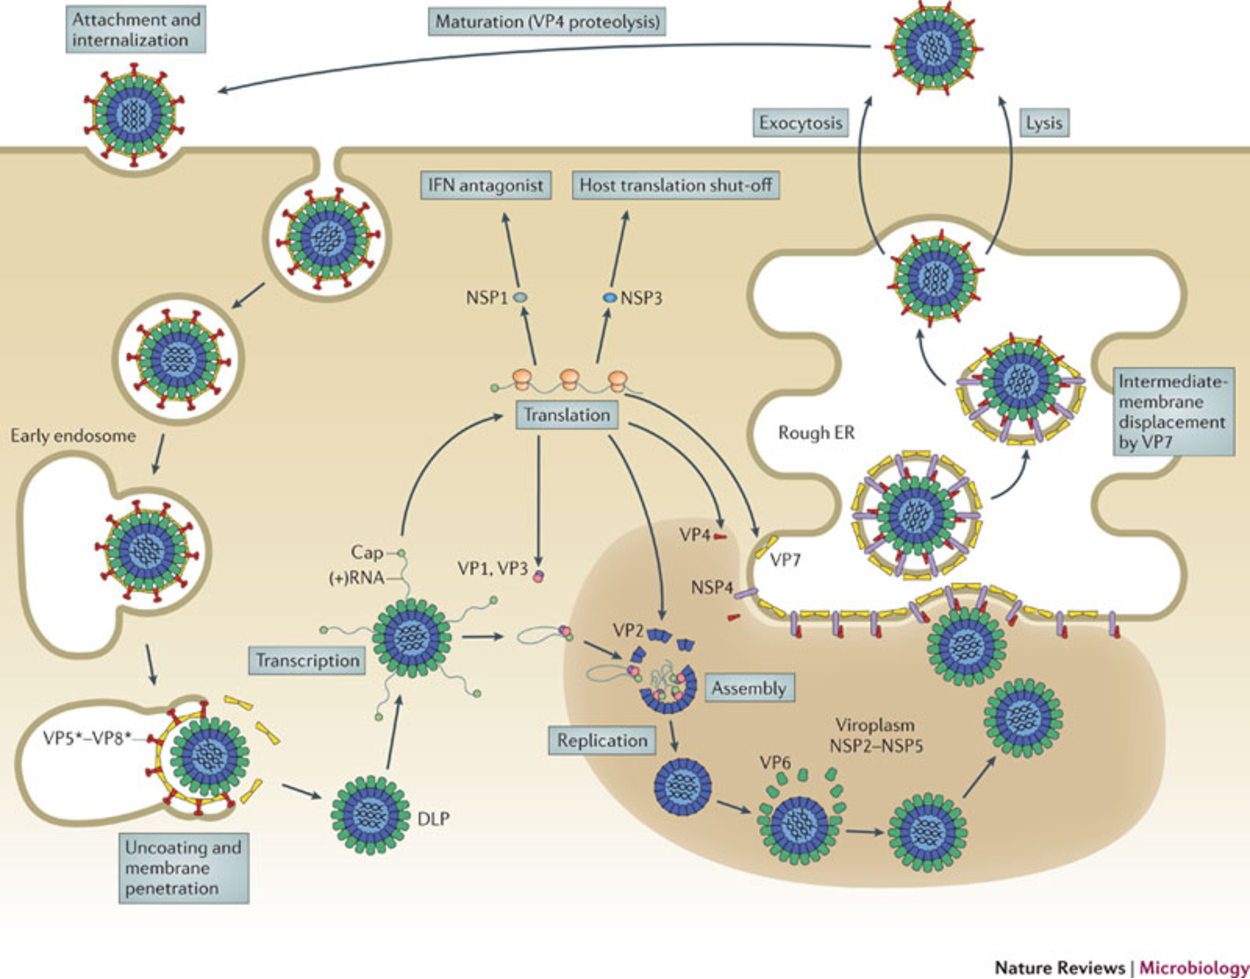
\includegraphics{replication}\\
\caption{Stylized representation of rotavirus replication.}
\end{figure}
\end{landscape}

\subsection{Pathogenesis and Pathology}

\subsection{Epidemiology}

\subsection{Immunity}

\subsection{Clinical Features and Diagnosis}

\subsection{Prevention and Control}
	\clearpage
	
	%!TEX root=../labNotes.tex

\section{September 2014}

\subsection*{02 September 2014}

\begin{enumerate}
	\item Prepared serum-free Medium 199
		\begin{enumerate}
			\item Supplemented $500$mL incomplete Medium 199 (incomplete M199) with $5$mL penicillin/streptomycin stock ($100$U/mL penicillin; $100\mu$g/mL streptomycin final concentration) and $1$mL $250\mu$g/mL amphotericin B stock ($0.25\mu$g/mL amphotericin B final concentration)
			\item Stored at $4^{\circ}$C
		\end{enumerate}
	\item Prepared complete Medium 199
		\begin{enumerate}
				\item Supplemented $500$mL incomplete M199 with $5$mL penicillin/streptomycin stock ($100$U/mL penicillin; $100\mu$g/mL streptomycin final concentration) and $1$mL $250\mu$g/mL amphotericin B stock ($0.25\mu$g/mL amphotericin B final concentration), $55$mL fetal bovine serum
				\item Stored at $4^{\circ}$C
		\end{enumerate}
	\item MA104 cell split --- Passage 59
		\begin{enumerate}
			\item A T75 flask was split by Shu from her maintained stock, labeled, and incubated at $37^{\circ}$C
		\end{enumerate}
\end{enumerate}

\subsection*{03 September 2014}

\begin{enumerate}
	\item Prepared 2x EMEM, serum-free
		\begin{enumerate}
			\item Supplemented $500$mL 2x EMEM stock with $10$mL $200$mM L-glutamine stock ($4$mM L-glutamine final concentration), $10$mL penicillin/streptomycin stock ($200$U/mL penicillin; $200\mu$g/mL streptomycin final concentration), and $1$mL $250\mu$g/mL amphotericin B stock ($0.5\mu$g/mL amphotericin B final concentration)
			\item Stored at $4^{\circ}$C
		\end{enumerate}
	\item Prepared $400$mL $1.2$\% agarose
		\begin{enumerate}
			\item Combined $4.8020$g SeaPlaque agar to $\sim 400$mL milli-Q-filtered water
			\item Autoclaved for $20$ minutes
			\item Stored at room temperature
		\end{enumerate}
\end{enumerate}
	%!TEX root=../virology.tex

\subsection*{09 September 2014}

\begin{enumerate}
	\item MA104 cell split --- Passage 60, from Passage 59, Flask A
		\begin{enumerate}
			\item Aspirated cell culture medium
			\item Rinsed cells in $10$mL 1x PBS; aspirated PBS
			\item Rinsed cells in $2$mL $0.05$\% trypsin; aspirated trypsin
			\item Bathed cells in $2$mL $0.05$\% trypsin
			\item Incubated cells at $37^{\circ}$C until all cells detached from flask
			\item Added $18$mL complete M199 to flask
			\item Added to $3$ T150 flasks $15$mL complete M199/$10$mL cell mix; $20$mL complete M199/$5$mL cell mix; and $20$mL complete M199/$5$mL cell mix. Respectively, flasks A, B, and C
			\item Gently shook flasks to distribute cells evenly
			\item Incubated at $37^{\circ}$C
		\end{enumerate}
\end{enumerate}

\subsection*{12 September 2014}

\begin{enumerate}
	\item Plated MA104 cells --- Passage 60, Flask A
		\begin{enumerate}
			\item Aspirated cell culture medium
			\item Rinsed cells in $10$mL 1x PBS; aspirated PBS
			\item Rinsed cells in $5$mL $0.05$\% trypsin; aspirated trypsin
			\item Bathed cells in $5$mL $0.05$\% trypsin
			\item Incubated cells at $37^{\circ}$C until all cells detached from flask
			\item Added $15$mL complete M199 to flask
			\item Took cell count by combining $10\mu$L cell mixture with $10\mu$L trypan blue:
			
				\begin{align*}
				\text{[cells]} &= \frac{3.91\e{5}\text{ cells}}{1\text{mL}} \\
				\frac{\text{cells}}{\text{flask}} &= \frac{3.91\e{5}\text{ cells}}{1\text{mL}} \cdot 20\text{mL} &= \frac{7.62\e{6}\text{ cells}}{20\text{mL}}\\
				\frac{\text{cells}}{10\text{mL cell mix}} &= \frac{7.62\e{6}\text{ cells}}{20\text{mL}}\cdot \frac{1}{2} &= \frac{3.81\e{6}\text{ cells}}{10\text{mL}}\\
				\frac{\text{cells}}{75\text{mL vial}} &= \frac{3.81\e{6}\text{ cells}}{75\text{mL}} &= \frac{5.08\e{4}\text{ cells}}{\text{mL}}\\
				\frac{\text{cells}}{3\text{mL well}} &= \frac{5.08\e{4}\text{ cells}}{\text{mL}} \cdot 3\text{mL} &= \frac{1.52\e{5}\text{ cells}}{\text{well}}\\
				\end{align*}
			\item Added $65$mL complete M199 and $10$mL cell mixture to $125$mL conical vial for final volume of $75$mL
			\item Transferred $3$mL solution to each well of 4 6-well plates
			\item Spread cells evenly by shaking
			\item Incubated at $37^{\circ}$C
		\end{enumerate}
\end{enumerate}
	%!TEX root=../virology.tex

\subsection*{15 September 2014}

\begin{enumerate}
	\item MA104 cell split --- Passage 61, from P60, Flask B
		\begin{enumerate}
			\item Aspirated cell culture medium
			\item Rinsed cells in $10$mL 1x PBS; aspirated PBS
			\item Rinsed cells in $5$mL $0.05$\% trypsin; aspirated trypsin
			\item Bathed cells in $5$mL $0.05$\% trypsin
			\item Incubated cells at $37^{\circ}$C until all cells detached from flask
			\item Added $15$mL complete M199 to flask
			\item Added to $3$ T150 flasks $22.5$mL complete M199/$2.5$mL cell mix; $22.5$mL complete M199/$2.5$mL cell mix; and $20$mL complete M199/$5$mL cell mix, respectively
			\item Gently shook flasks to distribute cells evenly
			\item Incubated at $37^{\circ}$C
		\end{enumerate}
		
	\item Prepared 1x PBS
		\begin{enumerate}
			\item Combined $80$mL 10x PBS and $720$mL milli-Q-filtered water in a $1$L graduated cylinder
			\item Transferred to a $1$L bottle
			\item Autoclaved for 30 minutes
			\item Stored at room temperature
		\end{enumerate}
		
	\item Rotavirus activation and series dilution for P60A plated cells
		\begin{enumerate}
			\item Combined $400\mu$L SA11 rotavirus stock and $2$mL trypsin
			\item Incubated for 1 hour in a $37^{\circ}$C water bath
			\item Added $2.7$mL serum-free M199 to each of 8 $15$mL tubes
			\item To the first tube, added $300\mu$L rotavirus solution to a final concentration of $10^{-1}$
			\item Mixed contents by vertex
			\item To the next tube, added $300\mu$L rotavirus solution from the previous tube to a final concentration of $10^{-2}$
			\item Mixed contents by vertex
			\item Repeated serially for the remaining tubes ending with a concentration of $10^{-8}$ in the final tube
			\item Stored at $4^{\circ}$C
		\end{enumerate}
\end{enumerate}

\subsection*{16 September 2014}

\begin{enumerate}
	\item Plated MA104 cells --- Passage 60, Flask C
		\begin{enumerate}
			\item Aspirated cell culture medium
			\item Rinsed cells in $10$mL 1x PBS; aspirated PBS
			\item Rinsed cells in $5$mL $0.05$\% trypsin; aspirated trypsin
			\item Bathed cells in $5$mL $0.05$\% trypsin
			\item Incubated cells at $37^{\circ}$C until all cells detached from flask
			\item Added $15$mL complete M199 to flask
			\item Took cell count by combining $10\mu$L cell mixture with $10\mu$L trypan blue:
			
				\begin{align*}
				\text{[cells]} &= \frac{2.16\e{5}\text{ cells}}{1\text{mL}} \\
				\frac{\text{cells}}{\text{flask}} &= \frac{2.16\e{5}\text{ cells}}{1\text{mL}} \cdot 20\text{mL} &= \frac{4.32\e{6}\text{ cells}}{20\text{mL}}\\
				\frac{\text{cells}}{10\text{mL cell mix}} &= \frac{4.32\e{6}\text{ cells}}{20\text{mL}}\cdot \frac{1}{2} &= \frac{2.16\e{6}\text{ cells}}{10\text{mL}}\\
				\frac{\text{cells}}{75\text{mL vial}} &= \frac{2.16\e{6}\text{ cells}}{75\text{mL}} &= \frac{2.88\e{4}\text{ cells}}{\text{mL}}\\
				\frac{\text{cells}}{3\text{mL well}} &= \frac{2.88\e{4}\text{ cells}}{\text{mL}} \cdot 3\text{mL} &= \frac{8.64\e{4}\text{ cells}}{\text{well}}\\
				\end{align*}
			\item Added $65$mL complete M199 and $10$mL cell mixture to $125$mL conical vial for final volume of $75$mL
			\item Transferred $3$mL solution to each well of 4 6-well plates
			\item Spread cells evenly by shaking
			\item Incubated at $37^{\circ}$C
		\end{enumerate}
	\item Rotavirus infection of P60A plated cells
		\begin{enumerate}
			\item Washed monolayer in each well twice with serum-free M199 by dumping
			\item Added $\sim1$mL rotaviral solution to wells in concentrations from $10^{-3}$ to $10^{-8}$ with 2 wells being infected at each concentration of rotavirus
			\item Spread cells evenly by shaking
			\item Incubated at $37^{\circ}$C for 1 hour
		\end{enumerate}
	\item Agarose overlay of P60A plated cells
		\begin{enumerate}
			\item Liquefied 1.2\% agarose by microwave and equilibrated to $55^{\circ}$C
			\item For each plate of cells, prepared 1 vial of $10$mL agarose, $10$mL 2x EMEM, $5\mu$L $2$mg/mL trypsin
			\item Aspirated cell culture medium from each well
			\item To each well, added $\sim3$mL agarose solution
			\item Let agarose solidify
			\item Incubated at $37^{\circ}$C
		\end{enumerate}
\end{enumerate}

\subsection*{19 September 2014}

\begin{enumerate}
	\item MA104 cell split --- Passage 62, from Passage 61, Flask A
		\begin{enumerate}
			\item Aspirated cell culture medium
			\item Rinsed cells in $10$mL 1x PBS; aspirated PBS
			\item Rinsed cells in $5$mL $0.05$\% trypsin; aspirated trypsin
			\item Bathed cells in $5$mL $0.05$\% trypsin
			\item Incubated cells at $37^{\circ}$C until all cells detached from flask
			\item Added $15$mL complete M199 to flask
			\item Added to $3$ T150 flasks $22.5$mL complete M199/$2.5$mL cell mix; $22.5$mL complete M199/$2.5$mL cell mix; and $20$mL complete M199/$5$mL cell mix, respectively
			\item Gently shook flasks to distribute cells evenly
			\item Incubated at $37^{\circ}$C
		\end{enumerate}
	\item Neutral red overlay of P60A plated cells
		\begin{enumerate}
			\item Prepared 2 vials, each with $7.5$mL 1.2\% agarose, $7.5$mL 2x EMEM, and $600\mu$L neutral red
			\item To each well of 2 6-well plates, added $\sim 1$mL prepared agarose solution (using 1 vial per plate)
			\item Let agarose solution solidify
			\item Incubated at $37^{\circ}$C for 4 hours
			\item Observed $3\e{6}$PFU/mL
		\end{enumerate}
\end{enumerate}
	%!TEX root=../virology.tex

\subsection*{21 September 2014}

\begin{enumerate}
	\item Rotavirus activation and series dilution for P60C plated cells
		\begin{enumerate}
			\item Combined $400\mu$L SA11 rotavirus stock and $2$mL trypsin
			\item Incubated for 1 hour in a $37^{\circ}$C water bath
			\item Added $2.7$mL serum-free M199 to each of 8 $15$mL tubes
			\item To the first tube, added $300\mu$L rotavirus solution to a final concentration of $10^{-1}$
			\item Mixed contents by vertex
			\item To the next tube, added $300\mu$L rotavirus solution from the previous tube to a final concentration of $10^{-2}$
			\item Mixed contents by vertex
			\item Repeated serially for the remaining tubes ending with a concentration of $10^{-8}$ in the final tube
			\item Stored at $4^{\circ}$C
		\end{enumerate}
\end{enumerate}

\subsection*{22 September 2014}

\begin{enumerate}
	\item Rotavirus infection of P60C plated cells
		\begin{enumerate}
			\item Washed monolayer in each well twice with serum-free M199 by dumping
			\item Added $\sim1$mL rotaviral solution to wells in concentrations from $10^{-3}$ to $10^{-8}$ with 2 wells being infected at each concentration of rotavirus
			\item Spread cells evenly by shaking
			\item Incubated at $37^{\circ}$C for 1 hour
		\end{enumerate}
	\item Agarose overlay of P60C plated cells
		\begin{enumerate}
			\item Liquefied 1.2\% agarose by microwave and equilibrated to $55^{\circ}$C
			\item For each plate of cells, prepared 1 vial of $10$mL agarose, $10$mL 2x EMEM, $5\mu$L $2$mg/mL trypsin
			\item Aspirated cell culture medium from each well
			\item To each well, added $\sim3$mL agarose solution
			\item Let agarose solidify
			\item Incubated at $37^{\circ}$C
		\end{enumerate}
\end{enumerate}

\subsection*{25 September 2014}

\begin{enumerate}
	\item Prepared complete Medium 199
		\begin{enumerate}
				\item Supplemented $500$mL incomplete M199 with $5$mL penicillin/streptomycin stock ($100$U/mL penicillin; $100\mu$g/mL streptomycin final concentration) and $1$mL $250\mu$g/mL amphotericin B stock ($0.25\mu$g/mL amphotericin B final concentration), $55$mL fetal bovine serum
				\item Stored at $4^{\circ}$C
		\end{enumerate}
	\item Plated MA104 cells --- Passage 61, Flask B
		\begin{enumerate}
			\item Aspirated cell culture medium
			\item Rinsed cells in $10$mL 1x PBS; aspirated PBS
			\item Rinsed cells in $5$mL $0.05$\% trypsin; aspirated trypsin
			\item Bathed cells in $5$mL $0.05$\% trypsin
			\item Incubated cells at $37^{\circ}$C until all cells detached from flask
			\item Added $15$mL complete M199 to flask
			\item Took cell count by combining $10\mu$L cell mixture with $10\mu$L trypan blue:
			
				\begin{align*}
				% Initial
				\text{[cells]} &= \frac{3.56\e{5}\text{ cells}}{1\text{mL}} \\
				% Cells / flask
				\frac{\text{cells}}{\text{flask}} &= \frac{3.56\e{5}\text{ cells}}{1\text{mL}} \cdot 20\text{mL} &= \frac{7.12\e{6}\text{ cells}}{20\text{mL}}\\
				% Cells / 10mL
				\frac{\text{cells}}{10\text{mL cell mix}} &= \frac{7.12\e{6}\text{ cells}}{20\text{mL}}\cdot \frac{1}{2} &= \frac{3.56\e{6}\text{ cells}}{10\text{mL}}\\
				% Cells / conical vial
				\frac{\text{cells}}{75\text{mL vial}} &= \frac{3.56\e{6}\text{ cells}}{75\text{mL}} &= \frac{4.75\e{4}\text{ cells}}{\text{mL}}\\
				% Cells / well
				\frac{\text{cells}}{3\text{mL well}} &= \frac{4.75\e{4}\text{ cells}}{\text{mL}} \cdot 3\text{mL} &= \frac{1.42\e{5}\text{ cells}}{\text{well}}\\
				\end{align*}
			\item Added $65$mL complete M199 and $10$mL cell mixture to $125$mL conical vial for final volume of $75$mL
			\item Transferred $3$mL solution to each well of 4 6-well plates
			\item Spread cells evenly by shaking
			\item Incubated at $37^{\circ}$C
		\end{enumerate}
	\item Neutral red overlay of P60C plated cells
		\begin{enumerate}
			\item Prepared 2 vials, each with $7.5$mL 1.2\% agarose, $7.5$mL 2x EMEM, and $600\mu$L neutral red
			\item To each well of 2 6-well plates, added $\sim 1$mL prepared agarose solution (using 1 vial per plate)
			\item Let agarose solution solidify
			\item Incubated at $37^{\circ}$C for 4 hours
			\item Agarose was applied too hot and plaques observed were not sufficient
		\end{enumerate}
\end{enumerate}

\subsection*{26 September 2014}

\begin{enumerate}
	\item Rotavirus activation and series dilution for P61B plated cells
		\begin{enumerate}
			\item Combined $400\mu$L SA11 rotavirus stock and $2$mL trypsin
			\item Incubated for 1 hour in a $37^{\circ}$C water bath
			\item Added $2.7$mL serum-free M199 to each of 8 $15$mL tubes
			\item To the first tube, added $300\mu$L rotavirus solution to a final concentration of $10^{-1}$
			\item Mixed contents by vertex
			\item To the next tube, added $300\mu$L rotavirus solution from the previous tube to a final concentration of $10^{-2}$
			\item Mixed contents by vertex
			\item Repeated serially for the remaining tubes ending with a concentration of $10^{-8}$ in the final tube
			\item Stored at $4^{\circ}$C
		\end{enumerate}
	\item MA104 cell split --- Passage 63, from Passage 62, Flask B
		\begin{enumerate}
			\item Aspirated cell culture medium
			\item Rinsed cells in $10$mL 1x PBS; aspirated PBS
			\item Rinsed cells in $5$mL $0.05$\% trypsin; aspirated trypsin
			\item Bathed cells in $5$mL $0.05$\% trypsin
			\item Incubated cells at $37^{\circ}$C until all cells detached from flask
			\item Added $15$mL complete M199 to flask
			\item Added to $3$ T150 flasks $20$mL complete M199/$5$mL cell mix; $22.5$mL complete M199/$2.5$mL cell mix; and $22.5$mL complete M199/$2.5$mL cell mix. Respectively, flasks A, B, and C
			\item Gently shook flasks to distribute cells evenly
			\item Incubated at $37^{\circ}$C
		\end{enumerate}
\end{enumerate}
	%!TEX root=../labNotes.tex

\subsection*{28 September 2014}

\begin{enumerate}
	\item Rotavirus infection of P61B plated cells
		\begin{enumerate}
			\item Washed monolayer in each well twice with serum-free M199 by dumping
			\item Added $\sim 1$mL rotaviral solution to wells in concentrations from $10^{-3}$ to $10^{-8}$ with 2 wells being infected at each concentration of rotavirus
			\item Spread cells evenly by shaking
			\item Incubated at $37^{\circ}$C for 1 hour
		\end{enumerate}
	\item Agarose overlay of P61B plated cells
		\begin{enumerate}
			\item Liquefied 1.2\% agarose by microwave and equilibrated to $55^{\circ}$C
			\item For each plate of cells, prepared 1 vial of $10$mL agarose, $10$mL 2x EMEM, $5\mu$L $2$mg/mL trypsin
			\item Aspirated viral inoculant from each well
			\item To each well, added $\sim3$mL agarose solution
			\item Let agarose solidify
			\item Incubated at $37^{\circ}$C
		\end{enumerate}
	\item Plated MA104 cells --- Passage 62, Flask C
		\begin{enumerate}
			\item Aspirated cell culture medium
			\item Rinsed cells in $10$mL 1x PBS; aspirated PBS
			\item Rinsed cells in $5$mL $0.05$\% trypsin; aspirated trypsin
			\item Bathed cells in $5$mL $0.05$\% trypsin
			\item Incubated cells at $37^{\circ}$C until all cells detached from flask
			\item Added $15$mL complete M199 to flask
			\item Took cell count by combining $10\mu$L cell mixture with $10\mu$L trypan blue:
			
				\begin{align*}
				% Initial
				\text{[cells]} &= \frac{4.16\e{5}\text{ cells}}{1\text{mL}} \\
				% Cells / flask
				\frac{\text{cells}}{\text{flask}} &= \frac{4.16\e{5}\text{ cells}}{1\text{mL}} \cdot 20\text{mL} &= \frac{8.32\e{6}\text{ cells}}{20\text{mL}}\\
				% Cells / 10mL
				\frac{\text{cells}}{10\text{mL cell mix}} &= \frac{8.32\e{6}\text{ cells}}{20\text{mL}}\cdot \frac{1}{2} &= \frac{4.16\e{6}\text{ cells}}{10\text{mL}}\\
				% Cells / conical vial
				\frac{\text{cells}}{75\text{mL vial}} &= \frac{4.16\e{6}\text{ cells}}{75\text{mL}} &= \frac{5.55\e{4}\text{ cells}}{\text{mL}}\\
				% Cells / well
				\frac{\text{cells}}{3\text{mL well}} &= \frac{5.55\e{4}\text{ cells}}{\text{mL}} \cdot 3\text{mL} &= \frac{1.67\e{5}\text{ cells}}{\text{well}}\\
				\end{align*}
			\item Added $65$mL complete M199 and $10$mL cell mixture to $125$mL conical vial for final volume of $75$mL
			\item Transferred $3$mL solution to each well of 4 6-well plates
			\item Spread cells evenly by shaking
			\item Incubated at $37^{\circ}$C
		\end{enumerate}
\end{enumerate}

\subsection*{29 September 2014}

\begin{enumerate}
	\item Lentiviral transduction of P62C plated cells
		\begin{enumerate}
			\item Counted cells per well
				\begin{enumerate}
					\item To one well, added $1$mL 1x PBS; aspirated
					\item Rinsed in $500\mu$L trypsin; aspirated
					\item Bathed in $500\mu$L trypsin
					\item Incubated at $37^{\circ}$C until cells detached
					\item Added $1.5$mL complete M199
					\item Took cell count by combining $10\mu$L cell mixture with $10\mu$L trypan blue:
			
					\begin{align*}
					% Initial
					\text{[cells]} &= \frac{9.03\e{4}\text{ cells}}{1\text{mL}} \\
					% Cells / well
					\frac{\text{cells}}{2\text{mL well}} &= \frac{9.05\e{4}\text{ cells}}{\text{mL}} \cdot 2\text{mL} &= \frac{1.86\e{5}\text{ cells}}{\text{well}}\\
					\end{align*}
				\end{enumerate}
			\item Calculated RIO3 dilution
				\begin{align*}
					% initial
					\text{[RIO3]} &= \frac{2.13\e{9}\text{ particles}}{1\text{mL}}\\
					% MOI = 10
					\text{dilution}&= \left(\frac{1.86\e{5}\text{ cells}}{\text{well}}\cdot \frac{10\text{ particles}}{1\text{ cell}}\right)/\frac{2.13\e{9}\text{ particles}}{1\text{mL}}\\
					&= \frac{0.87\mu\text{L}}{\text{well}}\\
					&= \frac{4.4\mu\text{L}}{5\text{ wells}}
				\end{align*}
			\item Calculated NSV dilution
				\begin{align*}
					% initial
					\text{[NSV]} &= \frac{1.95\e{8}\text{ particles}}{1\text{mL}}\\
					% MOI = 10
					\text{dilution}&= \left(\frac{1.86\e{5}\text{ cells}}{\text{well}}\cdot \frac{10\text{ particles}}{1\text{ cell}}\right)/\frac{1.95\e{8}\text{ particles}}{1\text{mL}}\\
					&= \frac{9.54\mu\text{L}}{\text{well}}\\
					&= \frac{47.7\mu\text{L}}{5\text{ wells}}
				\end{align*}
			\item Prepared RIO3 wells
				\begin{enumerate}
					\item Combined $5$mL complete M199, $5\mu$L polybreen, and $4.4\mu$L RIO3 and mixed by vertex
					\item Aspirated cell culture medium from experimental wells
					\item To each of the 5 experimental wells, added $1$mL RIO3 solution
					\item Spread evenly by gently shaking plates
				\end{enumerate}
			\item Prepared NSV control wells
				\begin{enumerate}
					\item Combined $5$mL complete M199, $5\mu$L polybreen, and $47.7\mu$L NSV and mixed by vertex
					\item Aspirated cell culture medium from control wells
					\item To each of the 5 control wells, added $1$mL NSV solution
					\item Spread evenly by gently shaking plates
				\end{enumerate}
			\item Incubated plates at $37^{\circ}$C for 2 hours
			\item Supplemented each of the 5 experimental wells with an additional $2$mL complete M199 ($3$mL final well volume)
			\item With a separate pipet, supplemented each of the 5 control wells with an additional $2$mL complete M199 ($3$mL final well volume)
			\item Incubated plates at $37^{\circ}$C
		\end{enumerate}
\end{enumerate}

\section{October 2014}

\subsection*{01 October 2014}

\begin{enumerate}
	\item Prepared serum-free Medium 199
		\begin{enumerate}
			\item Supplemented $500$mL incomplete M199 with $5$mL penicillin/streptomycin stock ($100$U/mL penicillin; $100\mu$g/mL streptomycin final concentration) and $1$mL $250\mu$g/mL amphotericin B stock ($0.25\mu$g/mL amphotericin B final concentration)
			\item Stored at $4^{\circ}$C
		\end{enumerate}
	\item Rotavirus infection of P62C plated cells (RIO3 and NSV transfected)
		\begin{enumerate}
			\item Counted cells per well
				\begin{enumerate}
					\item To one well, added $1$mL 1x PBS; aspirated
					\item Rinsed in $500\mu$L trypsin; aspirated
					\item Bathed in $500\mu$L trypsin
					\item Incubated at $37^{\circ}$C until cells detached
					\item Added $1.5$mL complete M199
					\item Took cell count by combining $10\mu$L cell mixture with $10\mu$L trypan blue:
			
					\begin{align*}
					% Initial
					\text{[cells]} &= \frac{1.18\e{5}\text{ cells}}{1\text{mL}} \\
					% Cells / well
					\frac{\text{cells}}{2\text{mL well}} &= \frac{1.18\e{5}\text{ cells}}{\text{mL}} \cdot 2\text{mL} &= \frac{2.36\e{5}\text{ cells}}{\text{well}}\\
					\end{align*}
				\end{enumerate}
			\item Calculated SA11 dilution
				\begin{align*}
					% initial
					\text{[SA11]} &= \frac{5\e{7}\text{ PFU}}{1\text{mL}}\\
					% MOI = 10
					\text{dilution}&= \left(\frac{2.36\e{5}\text{ cells}}{\text{well}}\cdot \frac{5\text{ particles}}{1\text{ cell}}\right)/\frac{5\e{7}\text{ PFU}}{1\text{mL}}\\
					&= \frac{23.6\mu\text{L}}{\text{well}}\\
					&= \frac{118\mu\text{L}}{5\text{ wells}}
				\end{align*}
			\item Prepared viral inoculant
				\begin{enumerate}
					\item To a vial, combined $400\mu$L SA11 and $2\mu$L trypsin
					\item Incubated in $37^{\circ}$C water bath for 1 hour
					\item Prepared vial of $10$mL serum-free M199
					\item Added to vial $236$mL viral solution (for infection of 10 wells)
				\end{enumerate}
			\item Washed wells twice with serum-free M199 by dumping
			\item Added to each well $1$mL viral solution
			\item Spread evenly by gently shaking plates
			\item Incubated plates at $37^{\circ}$C for 1 hour
			\item Aspirated viral inoculant from wells
			\item Added to each well $3$mL serum-free M199 and $0.75\mu$L trypsin
			\item Incubated plates at $37^{\circ}$C
		\end{enumerate}
	\item Plated MA104 cells --- Passage 63, Flask A
		%%%%%%%%%%%%%%%%%%%%%%%%%%%%%%
		% Go for a higher dilution --- these will be for more of
		% the *actual* exp runs, so we want 80% confluence
		% probably on Friday for LV transduction
		%%%%%%%%%%%%%%%%%%%%%%%%%%%%%%
		\begin{enumerate}
			\item Aspirated cell culture medium
			\item Rinsed cells in $10$mL 1x PBS; aspirated PBS
			\item Rinsed cells in $5$mL $0.05$\% trypsin; aspirated trypsin
			\item Bathed cells in $5$mL $0.05$\% trypsin
			\item Incubated cells at $37^{\circ}$C until all cells detached from flask
			\item Added $15$mL complete M199 to flask
			\item Took cell count by combining $10\mu$L cell mixture with $10\mu$L trypan blue:
			
				\begin{align*}
				% Initial
				\text{[cells]} &= \frac{4.61\e{5}\text{ cells}}{1\text{mL}} \\
				% Cells / flask
				\frac{\text{cells}}{\text{flask}} &= \frac{4.61\e{5}\text{ cells}}{1\text{mL}} \cdot 20\text{mL} &= \frac{9.22\e{6}\text{ cells}}{20\text{mL}}\\
				% Cells / 10mL
				\frac{\text{cells}}{10\text{mL cell mix}} &= \frac{9.22\e{6}\text{ cells}}{20\text{mL}}\cdot \frac{1}{2} &= \frac{4.61\e{6}\text{ cells}}{10\text{mL}}\\
				% Cells / conical vial
				\frac{\text{cells}}{75\text{mL vial}} &= \frac{4.61\e{6}\text{ cells}}{75\text{mL}} &= \frac{6.15\e{4}\text{ cells}}{\text{mL}}\\
				% Cells / well
				\frac{\text{cells}}{3\text{mL well}} &= \frac{6.15\e{4}\text{ cells}}{\text{mL}} \cdot 3\text{mL} &= \frac{1.84\e{5}\text{ cells}}{\text{well}}\\
				\end{align*}
			\item Added $65$mL complete M199 and $10$mL cell mixture to $125$mL conical vial for final volume of $75$mL
			\item Transferred $3$mL solution to each well of 4 6-well plates
			\item Spread cells evenly by shaking
			\item Incubated at $37^{\circ}$C
		\end{enumerate}
	\item Neutral red overlay of P62C plated cells
		\begin{enumerate}
			\item Prepared a vial with $7.5$mL 1.2\% agarose, $7.5$mL 2x EMEM, and $750\mu$L neutral red
			\item To each well of 2 6-well plates, added $\sim 1$mL prepared agarose solution
			\item Let agarose solution solidify
			\item Incubated at $37^{\circ}$C overnight
			\item Observed $\text{titer}=7\e{6}\text{ PFU/mL}$
		\end{enumerate}
\end{enumerate}

%%%%%%%%%%%%%%%%%%%%
% Thursday Plan
%%%%%%%%%%%%%%%%%%%%
% Probably split one flask (P63B),
% Bin the other (P63C)? Shoot for
% 3 1:8 dilutions so that there won't
% be much going on over the
% weekend, but we're good to get
% more runs in on Monday.
% Freeze transfected cells to lyse;
%%%%%%%%%%%%%%%%%%%%

\subsection*{02 October 2014}

\begin{enumerate}
	\item MA104 cell split --- Passage 64, from Passage 63, Flask B
		\begin{enumerate}
			\item Aspirated cell culture medium
			\item Rinsed cells in $10$mL 1x PBS; aspirated PBS
			\item Rinsed cells in $5$mL $0.05$\% trypsin; aspirated trypsin
			\item Bathed cells in $5$mL $0.05$\% trypsin
			\item Incubated cells at $37^{\circ}$C until all cells detached from flask
			\item Added $15$mL complete M199 to flask
			\item Added to $3$ T150 flasks $20$mL complete M199/$5$mL cell mix; $22.5$mL complete M199/$2.5$mL cell mix; and $22.5$mL complete M199/$2.5$mL cell mix. Respectively, flasks A, B, and C
			\item Gently shook flasks to distribute cells evenly
			\item Incubated at $37^{\circ}$C
		\end{enumerate}
	\item Lysed P62C transfected cells
		\begin{enumerate}
			\item Froze transfected cells in $-80^{\circ}$C freezer for 30 minutes; thawed
			\item Froze transfected cells in $-20^{\circ}$C freezer overnight
		\end{enumerate}
\end{enumerate}

%%%%%%%%%%%%%%%%%%%%
% Friday plan
%%%%%%%%%%%%%%%%%%%%
% Harvest RV from transfected cells
% Maybe infect plated cells?
%%%%%%%%%%%%%%%%%%%%

\subsection*{03 October 2014}

\begin{enumerate}
	\item Collected viral load from lysed P62C transfected cells
		\begin{enumerate}
			\item Thawed P62C cells
			\item Transferred content of each well to its own $15$mL tube
			\item Centrifuged tubes for 10 minutes at $500$RPM and $4^{\circ}$C
			\item Transfered supernatant from each centrifuged solution into fresh test tubes
			\item Stored at $-20^{\circ}$C
		\end{enumerate}
\end{enumerate}

\end{document}